\documentclass[11pt]{beamer}
\usetheme{Boadilla}
\usepackage[utf8]{inputenc}
\usepackage[english]{babel}
\usepackage{amsmath}
\usepackage{amsfonts}
\usepackage{amssymb}
\usepackage{graphicx}
\usepackage{tikz-cd}
\usepackage{tikz}
\usepackage{stmaryrd}

\tikzset{every path/.style={thick}}

\newtheorem{prop}[theorem]{Proposition}
\newtheorem{conjecture}[theorem]{Conjecture}

\theoremstyle{remark}
\newtheorem*{remark}{Remark}

\theoremstyle{remark}
\newtheorem*{slogan}{Slogan}

\newcommand{\Diff}{\operatorname{Diff}}
\newcommand{\Hom}{\operatorname{Hom}}
\newcommand{\End}{\operatorname{End}}
\newcommand{\Der}{\operatorname{Der}}
\newcommand{\coim}{\operatorname{coim}}
\newcommand{\im}{\operatorname{im}}
\newcommand{\coker}{\operatorname{coker}}
\newcommand{\id}{\textnormal{id}}
\newcommand{\N}{\mathbb{N}}
\newcommand{\Z}{\mathbb{Z}}
\newcommand{\Q}{\mathbb{Q}}
\newcommand{\R}{\mathbb{R}}
\newcommand{\C}{\mathbb{C}}
\newcommand{\A}{\mathbb{A}}
\newcommand{\F}{\mathbb{F}}
\newcommand{\I}{\mathrm{i}}
\renewcommand{\P}{\mathbb{P}}

\AtBeginSection[]
{
  \begin{frame}
    \frametitle{Table of Contents}
    \tableofcontents[currentsection]
  \end{frame}
}

\author{Lukas Johannsen}
\title{Quantum-classical duality}
%\setbeamercovered{transparent} 
%\setbeamertemplate{navigation symbols}{} 
%\logo{} 
\institute{University of Hamburg}
%\date{}
\begin{document}

\begin{frame}
\titlepage
\end{frame}

%\begin{frame}
%\tableofcontents
%\end{frame}

\section{State of the art}

\begin{frame}{State of the art}
It was observed by Gorsky, Zabrodin and Zotov \cite{article:gorsky:2014}, that the spectrum of the twist matrix $g$ of the quantum inhomogeneous Heisenberg model coincides with the spectrum of the Lax matrix $L$ of the classical rational Ruijsenaars-Schneider model under the following substitutions:

\begin{center}
\begin{tabular}{|l||l|}
\hline
$i$th particle & $i$th spin \\
position $y_i$ & inhomogeneity $y_i$ \\
velocity $\dot y_i$ & non-local Hamiltonian $H_i$ \\
\hline
\end{tabular}
\end{center}
The non-local Hamiltonians are given by
\begin{equation*}
H_i := \operatorname{Res}_{z=y_i} \tau^g(z),
\end{equation*}
where $\tau^g(z)$ denotes the $g$-twisted transfer matrix. We call this fact \emph{quantum-classical duality}.
\end{frame}

\begin{frame}{Functional relations}
Recently, Arutyunov \cite{book:arutyunov:betheAnsatz} formulated a system of polynomial equations for the spectrum of $H_1,...,H_N$ in terms of functional relations between higher transfer matrices $\tau_\lambda^g(z)$, where $\lambda$ is a Young diagram.

The basic functional relation is
\begin{equation*}
\tau_{[1^{k+1}]}(z) = \tau^g(z) \tau_{[1^k]}^g(z-\eta) - \tau_{[2,1^{k-1}]}(z-\eta),
\end{equation*}
from which we derive the recursion relation
\begin{equation*}
\operatorname{Res}_{z=y_i} \tau_{[1^{k+1}]}(z) = e_k(g) H_i + \sum_j \underset{\text{Lax matrix}}{\underbrace{\frac{\eta H_i}{y_i-y_j-\eta}}} \operatorname{Res}_{z=y_j} \tau_{[1^k]}(z).
\end{equation*}
We see the Lax matrix of the rational RS model appearing.
\end{frame}

\begin{frame}{Spectral equation}
Iterating the recursion relation and plugging in well-known eigenvalues of the quantum determinant
\begin{equation*}
\det g \operatorname{qdet} T(z) = \tau_{[1^\ell]}^g(z)
\end{equation*}
yields a Cayley-Hamilton-like identity consistent with \cite{article:gorsky:2014}:
\begin{equation*}
\sum_{k=0}^\ell e_k(g) L^k
\begin{pmatrix}
b_1 \\ \vdots \\ b_N
\end{pmatrix}
= 0,
\end{equation*}
where
\begin{equation*}
b_i := \prod_{i \neq j} \frac{y_i-y_j-\eta}{y_i-y_j}.
\end{equation*}
This system of $N$ equations of order $\ell$ form the \emph{spectral equations}.
\end{frame}

\section{QC duality as Schur-Weyl duality}

\begin{frame}{Representation theory}
These facts spark the quest for a deeper reason behind the correspondence between both models.
\\~\\
To this end, let us look at the representation theoretic structure of the Heisenberg model: The observables of the Heisenberg model live inside the Yangian $Y(\mathfrak{gl}_\ell)$ and its Hilbert space is given by the representation
\begin{equation*}
\C^\ell[y_1] \otimes \cdots \otimes \C^\ell[y_N]|_{y_i=u_i}.
\end{equation*}
This has a hidden symmetry given by the degenerate affine Hecke algebra
\begin{equation*}
\dot H_N = \C[S_N] \otimes \C[y_1,...,y_N]
\end{equation*}
via \emph{Schur-Weyl duality}.
\end{frame}

\begin{frame}{Schur-Weyl duality}
Schur-Weyl duality means that there is a bimodule structure
\begin{equation*}
Y(\mathfrak{gl}_\ell) \curvearrowright \C^\ell[y_1] \otimes \cdots \otimes \C^\ell[y_N] \curvearrowleft \dot H_N
\end{equation*}
that induces a functor
\begin{align*}
D_{\ell,N}: \dot H_N\mathsf{Mod} &\to Y(\mathfrak{gl}_\ell)\mathsf{Mod}, \\
U &\mapsto  (\C^\ell[y_1] \otimes \cdots \otimes \C^\ell[y_N]) \otimes_{\dot H_N} U,
\end{align*}
called the \emph{Drinfeld functor} \cite{article:drinfeld:1986}. This restricts to the well-known correspondence between representations of $S_N$ and $\mathfrak{gl}_\ell$.
\end{frame}

\begin{frame}{Quantum rational (spin) RS model}
There is a representation of $\dot H_N$ on polynomials $\C[y_1,..,y_N]$ that extends to a representation of the degenerate double affine Hecke algebra
\begin{equation*}
\ddot H_N := \C[X_1^{\pm 1},...,X_N^{\pm 1}] \otimes \C[S_N] \otimes \C[y_1,...,y_N].
\end{equation*}
The elementary symmetric polynomials $e_k(X_1,...,X_N)$ are commuting Hamiltonians for the quantum rational RS model.
\\~\\
We can then look at
\begin{equation*}
D_{\ell,N}(\C[y_1,...,y_N]) \cong (\C^\ell)^{\otimes N} \otimes_{S_N} \C[y_1,...,y_N],
\end{equation*}
which contains both the RS and Heisenberg model. It may be thought of as the Hilbert space of the rational \emph{spin} RS model, in analogy to \cite{article:lamers:2022}.
\end{frame}

\begin{frame}{Extending the Drinfeld functor}
We may extend and $g$-twist the Drinfeld functor, yielding
\begin{equation*}
D_{\ell,N}^g: \ddot H_N \to \ddot H_N^{S_N} \# Y(\mathfrak{gl}_\ell)\mathsf{Mod}.
\end{equation*}

\begin{theorem}[Quantum-classical duality]
The element
\begin{equation*}
\operatorname{tr} g + \sum_i \frac{\eta b_i X_i}{z-y_i} \in \ddot H_N^{S_N}\llbracket z^{-1} \rrbracket
\end{equation*}
acts on $D_{\ell,N}^g(\C[y_1,...,y_N])$ in the same way as $\tau^g(z)$ when $\hbar_{RS} = 0$.
\end{theorem}

\begin{slogan}
The $g$-twisted Drinfeld functor maps the Hamiltonians of the rational RS model to an $\hbar_{RS}$-deformation of the Hamiltonians of the Heisenberg model.
\end{slogan}
\end{frame}

\begin{frame}{Loop Yangian}
What happens when $\hbar_{RS} \neq 0$? Here we resort to a result of Guay \cite{article:guay:2005}, constructing a Schur-Weyl functor
\begin{equation*}
LD_{\ell,N}: \ddot H_N\mathsf{Mod} \to LY(\mathfrak{gl}_\ell)\mathsf{Mod},
\end{equation*}
where $LY(\mathfrak{gl}_\ell)$ is the \emph{loop Yangian}, which is a quotient of $L(\mathfrak{gl}_\ell) \# Y(\mathfrak{gl}_\ell)$ as well as $Y(\widehat{\mathfrak{gl}}_\ell)$.
\\~\\
\begin{theorem}
The loop variable $t$ living in the center of $L(\mathfrak{gl}_\ell)$ acts on $LD_{\ell,N}(\C[y_1,...,y_N])$ in the same way as the standard Hamiltonian of the rational RS model.
\end{theorem}
\end{frame}

\begin{frame}[fragile]{The full picture}
\begin{tikzpicture}[remember picture,overlay]
  \node[opacity=0.1] at (5.85cm,-4.3cm) {
    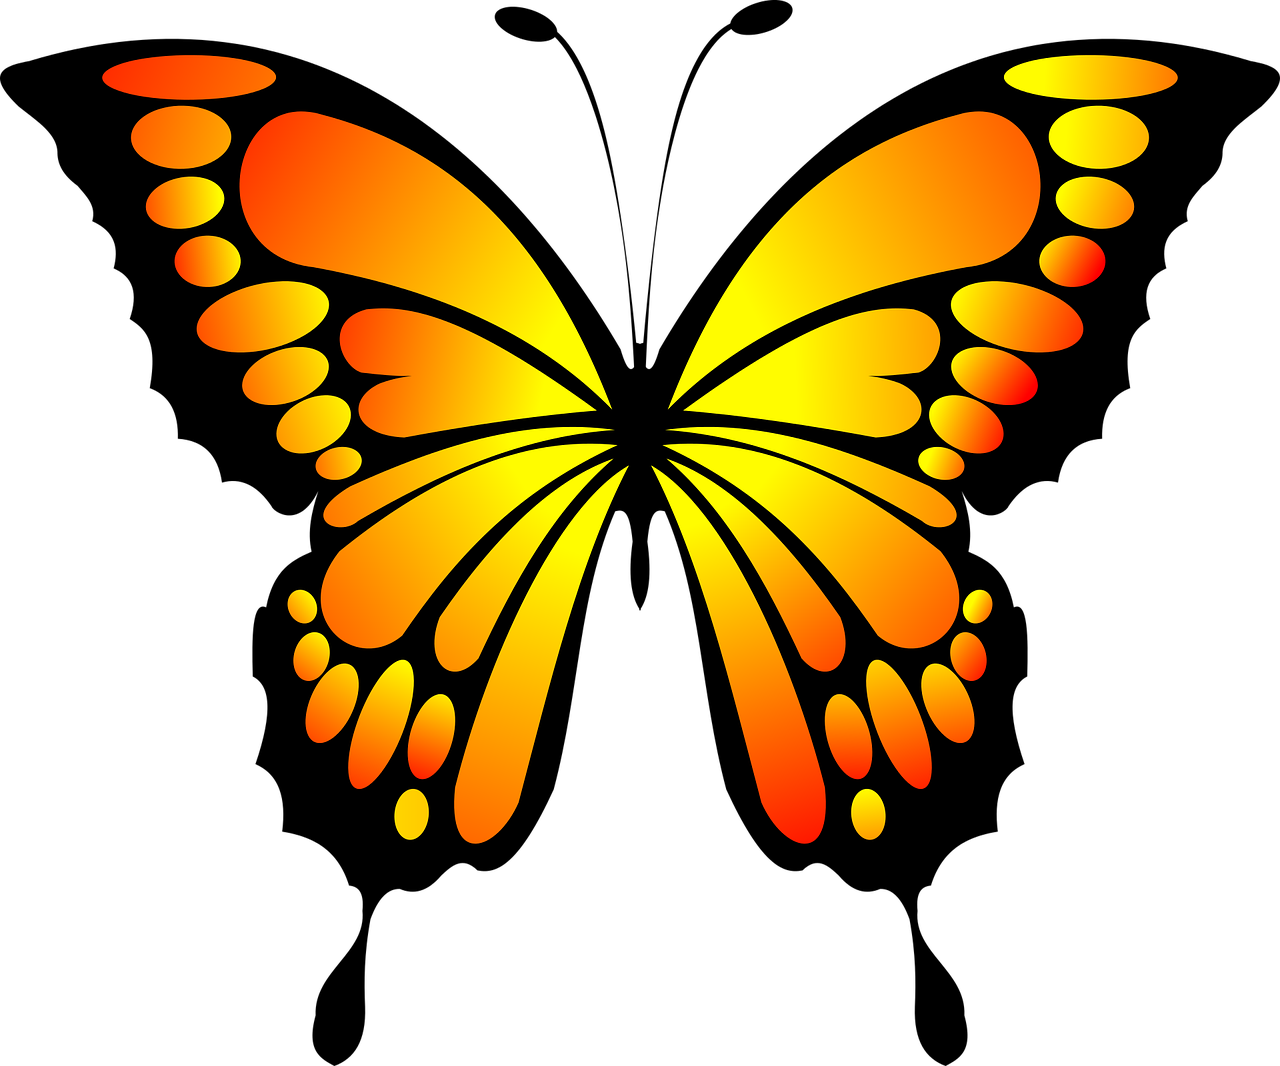
\includegraphics[width=10cm, height=6.5cm]{src/butterfly}
  };
\end{tikzpicture}
\begin{center}
\begin{tikzcd}[column sep=0.35cm,row sep=1.2cm]
\text{Heisenberg model} \arrow[leftrightarrow,bend right=50]{dd} \arrow[leftrightarrow,bend left=40]{rr} & & \text{trig. Gaudin model} \arrow[leftrightarrow,bend left=50]{dd} \\
 & \arrow[bend left=20]{ul} \arrow[bend right=20]{dl} LY(\mathfrak{gl}_\ell) \arrow[bend right=20]{ur} \arrow[bend left=20]{dr} & \\
\text{rat. RS model} \arrow[leftrightarrow,bend right=40]{rr} & & \text{trig. CM model}
\end{tikzcd}
\end{center}
\end{frame}

\begin{frame}{Comparison with classical models}
The loop Yangian $LY(\mathfrak{gl}_\ell)$ should be seen as the quantization of the Poisson structure found by Arutyunov and Frolov \cite{article:arutyunov:1998}:
\\~\\
They consider the rational spin RS and trigonometric spin CM models by Hamiltonian reduction of $T^* GL_N \times \mathfrak{gl}_N^*$ and derive two symmetries: The rational spin RS model has a loop symmetry and the trigonometric spin CM model has a Yangian symmetry.
\end{frame}

\section{QC duality in terms of 4d Chern-Simons theory}

\begin{frame}{4d Chern-Simons theory}
It is reasonable to ask for a geometric picture of the representation theoretic structures thus far. A natural guess where to look is 4d Chern-Simons theory, since it is known to assign the (delooping of the) category of representations of the Yangian to the formal punctured disc.
\\~\\
4d Chern-Simons theory is defined for a $\mathfrak{gl}_\ell$-gauge field $A$ on a 4-manifold $C \times \Sigma$, where $C$ is a complex curve equipped with a meromorphic 1-form $\omega$ and $\Sigma$ is an oriented surface. In our case, we look at $C = \P^1$ with $\omega = dz$ and $\Sigma = S^1 \times [0,1]$.
\\~\\
It was realized by Costello \cite{article:costello:2013} that Wilson lines along $S^1 \times [0,1]$ with constant coordinate in $\P^1$ recover the Heisenberg model.
\end{frame}

\begin{frame}[fragile]{Double category of cobordisms}
Such Wilson lines organize into a double category of cobordisms. Its objects are finite disjoint unions of $D^\times \times S_*^1$ and it has two types of morphisms: The first are purely topological cobordisms, such as
\begin{center}
\begin{tikzpicture}
\draw[red,dashed] (-0.5,-0.5) -- (-0.5,0.5);
%\node at (-1.5,0) {$X_2 =$};
\draw (-0.5,0) -- (0.5,0);
\draw (0.25,-0.5) -- (0.25,0.5);
%\draw (0.15,0) arc (0:90:0.15);
%\node[below] at (0,-0.5) {$y_1$};
\draw (0.5,0) .. controls (1,0) .. (1,0.5);
\draw (1,-0.5) .. controls (1,0) .. (1.5,0);
%\draw (1.5,0) -- (1.7,0);
%\node[below] at (1,-0.5) {$y_2$};
%\node at (2,0) {$\cdots$};
\draw (1.5,0) -- (2.5,0);
\draw (1.75,-0.5) -- (1.75,0.5);
%\draw (3.15,0) arc (0:90:0.15);
%\node[below] at (3,-0.5) {$y_N$};
\draw[red,dashed] (2.5,-0.5) -- (2.5,0.5);
\node[right] at (2.75,0.35) {$(S^1 \times [1,0])^{\sqcup 3}$};
\end{tikzpicture}
\end{center}
the second are purely holomorphic cobordisms
\begin{center}
\begin{tikzpicture}
\draw (0,0) circle (1cm);
\filldraw (0.45,-0.5) circle (1pt);
\node[above] at (0.45,-0.5) {$y_1$};
\filldraw (0,-0.65) circle (1pt);
\node[above] at (0,-0.55) {$y_2$};
\filldraw (-0.45,-0.5) circle (1pt);
\node[above] at (-0.45,-0.5) {$y_3$};
\filldraw (0,0.65) circle (1pt);
\node[below] at (0,0.65) {$\infty$};
\node[right] at (1,0.9) {$\P^1$};
\end{tikzpicture}
\end{center}
where we allow $y_1,...,y_N \in \P^1 \setminus \{ \infty \}$ with $y_i-y_j \neq 0,\eta$. Denote the space of such cobordisms by $Y_N$.
\end{frame}

\begin{frame}{QC duality in terms of 4d CS theory}
\begin{prop}
Quasi-coherent sheaves on $Y_N$ are equivalently modules over
\begin{equation*}
\underline{\dot H}_N := \dot H_N[(y_i-y_j)^{-1},(y_i-y_j-\eta)^{-1}].
\end{equation*}
\end{prop}
With this identification, we can view the Drinfeld functor as a functor
\begin{equation*}
\mathsf{Qcoh}(Y_N) \to Y(\mathfrak{gl}_\ell)\mathsf{Mod},
\end{equation*}
giving the part of 4d Chern-Simons theory that assigns Yangian modules to $\P^1 \times S^1$ with $N$ distinguished points on which Wilson lines may end.
\\~\\
I expect that the full picture in terms of the loop Yangian is recovered from 5d Chern-Simons theory on $\C \times \C^\times \times [0,1]$.
\end{frame}

\section{Towards a quantum elliptic spin RS model}

\begin{frame}{4d CS on $E \times S^1 \times [0,1]$}
The above considerations motivate the study of 4d Chern-Simons theory on $E \times S^1 \times [0,1]$, where $E = \C/\Lambda$ is an elliptic curve. We similarly look at configurations of points $Y_N^\text{ell}$ and let $\underline{\dot H}_N^\text{ell}$ denote the algebra whose modules model quasi-coherent sheaves on $Y_N^\text{ell}$. I expect that there is a Schur-Weyl bimodule
\begin{equation*}
E(\mathfrak{gl}_\ell) \curvearrowright (\C^\ell)^{\otimes N} \otimes \mathcal{O}(Y_N^\text{ell}) \curvearrowleft \underline{\dot H}_N^\text{ell}.
\end{equation*}
where $E(\mathfrak{gl}_\ell)$ is Belavin's elliptic quantum group \cite{article:costello:2018b,article:etingof:1998}. Tensoring with $\mathcal{O}(Y_N^\text{ell})$ over $\underline{\dot H}_N^\text{ell}$ should give the Hilbert space for the elliptic spin RS model. Its Hamiltonians will be elliptic difference operators deforming the residues of the elliptic transfer matrix.
\\~\\
The full picture comes from 5d Chern-Simons theory on $E \times \C^\times \times [0,1]$ and an elliptic quantum group for $\widehat{\mathfrak{gl}}_\ell$.
\end{frame}

\begin{frame}[allowframebreaks]
\bibliographystyle{alphaurl}
\bibliography{bibliography.bib}
\end{frame}
\end{document}